System architecture was defined as the elements or components contained within a system and their relationships in Sec.~\ref{sec:ch1:architecture} \cite{Crawley2004a, Mittal1989a, Wyatt2014a}. 
Designing breakthrough engineering systems with new capabilities and new levels of performance requires innovations in system architecture \cite{Cagan2005a, Chakrabarti2011a}.
Engineers often rely on heuristics such as design by analogy \cite{Chan2011a} and intuition when considering system architecture, but this may result in fixation on example designs and stifle innovation \cite{Linsey2010a}. 

Consider the following architecture design problem formulation:
\begin{subequations}
\label{eq:ch2:arch_outerloop}
\begin{align}
\min_{\bm{x}_a} \quad & \Psi(\bm{x}_a) \\
\text{subject to:} \quad & f_a(\bm{x}_a) = a \in \mathcal{F}_a
\end{align}
\end{subequations}

\noindent where $\gls{x}_{a}$ represents architecture design variables, $\gls{f}_a(\bm{x}_a)$ is a mapping between the architecture design variables and the architecture $\glsfoo[noindex]{architecture}$, and $\gls{objective}$ is a performance index. A fair comparison between architecture candidates in the set of feasible architectures $\gls{feasible}_a$ requires knowledge of the best possible performance for each candidate architecture. This requires optimization with respect to \textit{inner-loop} design variables such as plant and control design (see Chapter~\ref{ch:3}) \cite{Deshmukh2015a, Herber2017b}. The number design variables, constraints, models, etc.~can all change depending on the candidate architecture in the inner loop. Hence, formulating and solving architecture design problems can be challenging. Here we focus on a method that generates candidate architectures that may be used to determine the performance index with respect to an architecture-dependent inner-loop design problem.

Many studies have concentrated on effective representation and generation methods, primarily based on graph representations of the system architecture (see Fig.~\ref{fig:ch2:initialexamples} for some common engineering systems represented as graphs). There is a wide range of architecture design representations typically classified along the spectrum of continuum \cite{Hooshmand2012a, Khetan2015a} vs. discrete \cite{Munzer2013a, Guo2014a} design domains and homogeneous \cite{Hooshmand2012a, Khetan2015a} vs. heterogeneous \cite{Schmidt1997a, Munzer2013a} elements. The value of these methods often is to present new valid topologies to engineers for further evaluation (subjective or quantitative), helping to overcome design fixation. A popular class of methods for generating architecture candidates is generative representations \cite{Schmidt1997a, Schmidt2000a, Hornby2003a, Bryant2005a,  Hooshmand2012a,  Starling2005a, Chakrabarti2011a, Guo2014a}. This class covers a range of candidate architectures in an implicit form based on repeated application of rules that modify the graph. It has been recognized that generative approaches generate topologically simple designs, not covering the entire design space \cite{Munzer2013a}. Furthermore, the design space is sensitive to design knowledge \cite{Bryant2005a, Chan2011a} and rules \cite{Hooshmand2012a, Starling2005a}. While these designs may satisfy functional requirements elegantly, generation of more elaborate architectures is needed in some cases.

\begin{figure*}
\centering

\begin{subfigure}[b]{0.33\textwidth}
\centering
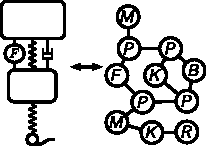
\includegraphics[scale=1]{../ch2/figures/suspension_optimized}
\caption{Suspension. \label{fig:ch2:initialexamples1}}
\end{subfigure}%
\begin{subfigure}[b]{0.33\textwidth}
\centering
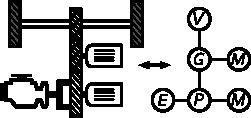
\includegraphics[scale=1]{../ch2/figures/powertrain_optimized}
\caption{Hybrid powertrain. \label{fig:ch2:initialexamples2}}
\end{subfigure}%
\begin{subfigure}[b]{0.33\textwidth}
\centering
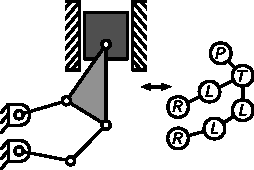
\includegraphics[scale=1]{../ch2/figures/linkage_optimized}
\caption{Mechanism. \label{fig:ch2:initialexamples3}}
\end{subfigure}

\vspace{0.05in}

\begin{subfigure}[b]{0.6\textwidth}
\centering
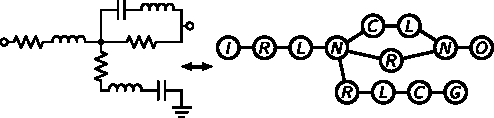
\includegraphics[scale=1]{../ch2/figures/circuit}
\caption{Electrical circuit.\label{fig:ch2:initialexamples4}}
\end{subfigure}%
\begin{subfigure}[b]{0.4\textwidth}
\centering

\includegraphics[scale=1]{../ch2/figures/molecule2}
\caption{Molecule.\label{fig:ch2:initialexamples5}}
\end{subfigure}

\caption{Architectures represented as graphs.\label{fig:ch2:initialexamples}}

\end{figure*}

It can be challenging to describe the design space of an architecture generation method, partially due to the combinatorial nature of architecture design problems. A better understanding of how certain rules restrict the design space can lead to better generative approaches, but this requires a complete design space to compare against. Furthermore, the ultimate goal is a set of all architectures that are feasible with respect to constraints \cite{Wyatt2012a} and that are unique \cite{Schmidt2000a}.  Arriving at such a design space efficiently is a considerable challenge.

In this chapter, the design space is completely captured by a perfect matchings approach for a certain class of architecture design problems, more specifically, problems that are represented by undirected colored graphs under the component/port paradigm \cite{Mittal1989a, Snavely1993a, Munzer2013a}.
The proposed approach generates truly novel architectures (in fact all of them) but still leverages some of the natural constraints found in architecture design problems to reduce the number of graphs generated.
This design space is found through an enumeration, i.e., a complete, ordered listing of all the items in the collection of feasible and unique architectures.
This approach leads to a number of interesting insights into the fundamental nature of architecture design problems.

The remainder of the chapter is organized as follows.
The next section outlines the some of the basic theory behind candidate architectures with perfect matchings.
Network structure constraints and the colored graph isomorphism problem are then discussed, with the objective of achieving feasible unique architectures.
Using the insights from the previous two sections, a tree search algorithm is developed that more efficiently covers the same design space.
A number of case studies are then presented.
Finally, a discussion is given of the results and how the proposed approaches can be used in current architecture design research.